\documentclass[../main]{subfiles}

\begin{document}

\section{Dual Optimization}\label{sec:dual}


\subsection{Conditions for strong
  duality}\label{sec:dual.conditions-for-strong-duality}


% \begin{theorem}
%   if \(\Omega_y\) is convex then the strong duality holds ...,
%   i.e.~\(\phi^\star = f^\star\)
% \end{theorem}

% add justifications here (slater, ...)

% A more interesting result is devoted to mixed integer problems.
Suppose \(\Omega_y\) is a mixed-integer set. We know Lagrangian relaxation produces a bound up to
continuous relaxation of a problem on convex hull of \(\Omega_y\) and relaxed constraints.

\textbf{(Review Here)}.

\begin{lemma}\label{lemma.bound}
  Suppose \(\Omega_y = \{y \in \mathbb R^n: y \in \Omega, y\in \mathbb Z^n\}\) and
  \(f=p^\mathsf{T}\delta + h^\mathsf{T} \epsilon\).
  Then we have the following relation for dual function,
  \[ \phi^\star = \min f(\delta, \epsilon)\quad \textbf{ s.t. }  y + \delta - \epsilon = b,\; y \in \textsf{conv}(\Omega_y)\]
\end{lemma}

The above lemma immediately allows us to have strong duality by definition of perfect formulation. We first define set \(Y\) be the intersection of the hyperplane and \(\textsf{conv}(\Omega_y)\),

\begin{equation}
  Y = \{(y, \delta, \epsilon): y + \delta - \epsilon = b,\; y \in \textsf{conv}(\Omega_y)\}
\end{equation}

Then we have the following results,

\begin{corollary}\label{lemma.strong-ip}
  We conclude the strong duality holds since \(Y\) is already \emph{a perfect formulation} in the sense that
  \(Y = \textsf{conv}(Y)\).
\end{corollary}

We conclude \(\phi^\star = f^\star\) since
\(f^\star = \min_{(y, \delta, \epsilon) \in \textsf{conv}(Y)} f(\delta, \epsilon)\).

\subsection{Subgradient Method}\label{sec:dual.subgradient}
As mentioned before, we assume the dual problem \(\phi(\lambda)\) can be solved efficiently \(\forall \lambda\).
To update the multiplier $\lambda$, we consider a class of subgradient
methods:

\begin{equation}\label{eq:main_subgrad}
  \lambda_{k+1} = \mathbf{P}(\lambda_{k} + s_{k}d_{k})
\end{equation}

where \(\mathbf P\) is the projection onto dual space \(\Lambda\), in the affine case \eqref{eq:def_affine}, we compute the projection onto \(n\)-dimensional box \(\Lambda = [-p, h]\).
\(d_k\) is the update direction for current iteration and \(s_{k}\) is
the step size using target-based rule:

\begin{equation}\label{eq:step_size}
  s_{k} = \gamma_k\frac{\phi^\star - \phi(\lambda_k)}{\|d_{k}\|^2}
\end{equation}

In practice, we take primal feasible values that are over estimates of \(\phi^\star\).

During the progress on dual problem,
we compute an weighted average solution \(\bar y_k\) from the convex combination of previous iterations:
\(\{y_i\}_{i=1,...k}\) and each \(y_i\) solves \(\phi_i = \phi(\lambda_i)\),
\(y_i = \arg\min_{y\in \Omega_y} \lambda_i^\mathsf{T}y\).

\begin{align}
  \label{eq:bar_y_average} \bar y_k & = \sum^i_k \alpha_i^{(k)} y_i,\quad  \sum^i_k \alpha_i^{(k)} = 1,\alpha_i^{(k)} \ge 0 \\
  \label{eq:bar_y_recursive}        & = (1-\alpha_k)\cdot\bar y_{k-1} + \alpha_k \cdot y_k
\end{align}

The second equation \eqref{eq:bar_y_recursive} rephrases the convexity in a recursive manner that may help in programming.
By taking \(g_k= y_k - b\), then \(g_k\) is a subgradient
of \(\phi\) at \(\lambda_k\):

\begin{equation}g_k \in \partial \phi_k\end{equation}


The search direction can be computed from subgradient.

\begin{equation}\label{eq:simple_subgrad}
  \begin{aligned}
     & \lambda_{k+1} = \mathbf{P}(\lambda_{k} + s_{k}g_{k})             \\
     & s_{k} = \gamma_k\frac{\phi^\star - \phi(\lambda_k)}{\|g_{k}\|^2}
  \end{aligned}
\end{equation}

As a comparison, we can use a convex alternative such that \(d_k = \bar y_k - b\).
Similarly, it can be expressed as convex combinations.
\begin{equation}\label{eq:direction_recursive}
  d_k = (1-\alpha_k) \cdot d_{k-1} + \alpha_k\cdot g_k
\end{equation}

For simplicity, we refer to the convex choice \eqref{eq:direction_recursive} whenever term \(d_k\) is used.

The dual subgradient algorithm can be summarized as follows.
\(\varepsilon,\varepsilon_s\) are the tolerance parameter for objective gap and stepsize, respectively.
\(\varepsilon > 0 ,\varepsilon_s > 0\). At each iteration \(k\), let \(\gamma_k < 2, \alpha_k = \frac{1}{k}\).

\begin{algorithm}[H]\label{alg:subgradient}
  \SetAlgoLined
  Initialization. \(\alpha_0 = 1, \lambda_0 = e, \gamma_0 = 1\)  \\
  \While{\(\phi^\star - \phi_k \ge \varepsilon\) \textbf{and} \(s_k \ge \varepsilon_s\)}
  {
    Let current iteration be \(k\)\\
    Update the multipliers by direction and stepsize, either by \eqref{eq:main_subgrad}, \eqref{eq:step_size} or \eqref{eq:simple_subgrad}.

    Solve dual problem \(\phi_k\) by \eqref{eq:dual}
    and compute subgradient \(g_k\) respectively.
  }
  \caption{The Subgradient Algorithm}
\end{algorithm}

It is obvious to see the solutions during dual optimization
\((y, \epsilon, \delta) = (y_k, 0, 0)\) are feasible if and only if we
can find \(y_k = d\), which in general will not hold. This motivates the following
algorithm based on linear programming theory.

\begin{algorithm}[H]\label{alg:recovery}
  \SetAlgoLined
  \begin{equation}\label{eq:recovery}
    \begin{aligned}
       & \epsilon_k = \max\{y_k - b, 0\}           \\
       & \delta_k = \max\{b - y_k, 0\}             \\
       & \bar \epsilon_k = \max\{\bar y_k - b, 0\} \\
       & \bar \delta_k = \max\{b - \bar y_k, 0\}
    \end{aligned}\end{equation}
  \caption{Recovery Algorithm}
\end{algorithm}

To simplify our presentation, let
\(z\) be the function of \(y\) for recovery algorithm \eqref{eq:recovery} such that \(z_k = z(y_k) = f(\delta_k, \epsilon_k)\), then \(z\) is
also convex in \(y\) since both function \(f\) and \(\max\{\cdot, 0\}\)
are convex. It's also worth to notice that \(\bar \epsilon_k\) should
not be calculated as running averages:
\(\bar \epsilon_k \neq \sum^i_k \alpha_i^{(k)} \epsilon_i\). For such an
``averaged'' solution, we let
\(\bar z_k = z(\bar y_k)\). We later find the recovery algorithm achieves
at the optimal objective.

\subsection{Overview}\label{sec:dual.overview}


We first review several features for the subgradient method regarding
parameters \(\gamma_k, \alpha_k\) and search direction \(d_k\) produced from convex combinations.

The target based rule are well-known as the Polyak rule \cite{polyak_general_1967}.
The idea of using previous searching directions is introduced to accelerate the subgradient method and provide a better stopping criterion,
see \cite{camerini_improving_1975}, \cite{brannlund_generalized_1995}, \cite{barahona_volume_2000}.
\cite{brannlund_generalized_1995} showed that with convex combinations the optimal choice of stepsize is
equivalent to the Camerini-Fratta-Maffioli modification, it also provides an analysis on its linear convergence rate.

From the primal perspective, our method is close to \emph{primal
  averaging method}. \cite{nedic_approximate_2009}
gives a line of analysis on convergence and quality of the primal
approximation by averaging over all previous solutions with a constant
stepsize. They use a simple averaging scheme with \(\alpha_k = 1/k\),
then it gives lower and upper bounds for the averaged solution
that involve the primal violation, norm of the subgradient, etc. Furthermore, they only analyze the case for constant
stepsize \(s_k = s, s\ge 0\) and the search direction defined solely by
the subgradient. We refer to \cite{kiwiel_lagrangian_2007} for target based
stepsizes. The volume algorithm proposed by \cite{barahona_volume_2000} is close to the
case mentioned in \cite{brannlund_generalized_1995} in a dual
viewpoint while adopting \(\tilde \lambda_{k}\) instead of \(\lambda_k\) from the best dual bound
\(\tilde \phi_k = \max_{i=1, ..., k} \phi(\lambda_i)\):

\[\lambda_{k+1} = \mathbf{P}(\tilde\lambda_{k} + s_{k}d_{k})\]

Since the solution is strictly feasible by implementation of the
recovery algorithm \eqref{eq:recovery}, i.e., there is no need to bound for feasibility gap
as has been done in most of literature covering the \textbf{primal
  recovery}. Instead, we focus on the quality of the recovery, i.e.:

\[
  |\bar z_k - \phi_k| \textrm { or } |\bar z_k - z^\star|
\]

We found its convergence is closely related to strong duality of the problem.

\subsection{Convergence Analysis}\label{dual.analysis}

Comments:

1. From Lemma \ref{lemma.bound} and Corollary \ref{lemma.strong-ip}, we see \(\phi^\star = f^\star\).

2. We assume convergence of dual method: \(\lambda_k \to \lambda^\star\), we don't limit our choice of subgradient method here. (computations has been done for using \(g_k\) or \(d_k\))

3. Simple recovery by using \(k\)-th solution, \(z_k = z(y_k)\), will not be convergent, see the \emph{green} lines in Figure \ref{fig:divergent_volume}, nor will the one using \(\min_k z(y_k)\).

4. Averaged recovery with \(\bar y_k\) and its value \(z(\bar y_k)\) is convergent, see the \emph{orange} lines. It is feasible to continuous relaxation (may not be integral). We expect its convergence to \(\phi^\star\).

% This part is only needed 
%   if use d_k (convex direction)
% \begin{lemma}\(\epsilon\)-subgradient.
%   \begin{equation}\label{eq:subgrad}
%     \begin{aligned}
%       g_{k}^\mathsf{T}(\lambda_{k}  -\lambda) \le \phi_{k} - \phi(\lambda) \\
%       d_{k}^\mathsf{T}(\lambda_{k}  -\lambda) \le \phi_{k} - \phi(\lambda) + \epsilon_k
%     \end{aligned}
%   \end{equation}
% \end{lemma}

% where

% \begin{equation}\label{eq:def_eps}
%   \epsilon_k = \sum^i_k \alpha^i_k \cdot \left [g_i^\mathsf{T}(\lambda_k - \lambda_i) + \phi_i - \phi_k \right ]
% \end{equation}

% Notice \(\epsilon_k\) can be further simplified by the definition of
% \(\phi\):

% \begin{equation}\label{eq:def_eps_simple}
%   \epsilon_k = \sum^i_k \alpha^i_k \cdot \left ( g_i^\mathsf{T}\lambda_k  - \phi_k \right )
% \end{equation}

% \begin{lemma} \label{lemma:dual_conv} Dual convergence, \cite{brannlund1995generalized}. The
%   subgradient method is convergent if \(\epsilon_k\) satisfies:
%   \begin{equation}
%     \frac{1}{2}(2 - \gamma_k) (\phi_{k} - \phi^\star)  + \epsilon_k \le 0
%   \end{equation}
% \end{lemma}
% \begin{proof}
%   The proof can be done by showing the monotonic decrease of
%   \(\|\lambda_{k} - \lambda^\star\|\) via the iterative equations.
%   \begin{equation}\begin{aligned}
%       \|\lambda_{k+1} - \lambda^\star\|^2 \le ||\lambda_k - \lambda^\star||^2
%       + 2\cdot \gamma_k \frac{(\phi^\star - \phi_{k})}{\|d_{k}\|^{2}} d_k^\mathsf{T}(\lambda_k - \lambda^\star)
%       + (\gamma_{k})^{2} \frac{(\phi^\star - \phi_{k})^{2}}{\|d_{k}\|^{2}}
%     \end{aligned}\end{equation}

%   Notice: \begin{equation}\begin{aligned}
%           & 2  \cdot d_k^\mathsf{T}(\lambda_k - \lambda^\star) + \gamma_{k}(\phi^\star - \phi_{k})
%       \le & 2 (\phi_{k} - \phi^\star + \epsilon_k) + \gamma_k(\phi^\star -\phi_k)                  \\
%       =   & (2 - \gamma_k) (\phi_{k} - \phi^\star)  + 2\epsilon_k \le 0
%     \end{aligned}\end{equation}

%   and we have the convergence.
% \end{proof}


Now we visit properties for primal solutions.

\begin{theorem} \label{lemma:recovery}  Recovery Algorithm \eqref{eq:recovery}
  \begin{enumerate}
    \def\labelenumi{(\alph{enumi})}

    \item
          For fixed \(y=y_k\), \((\epsilon_k, \delta_k)\) is the optimal
          solution for the restricted primal problem.
  \end{enumerate}

  \[f(\epsilon_k, \delta_k) \le f(\epsilon, \delta), \quad \forall \delta\ge 0, \epsilon\ge 0, y= y_k\]

  % \begin{enumerate}
  %   \def\labelenumi{(\alph{enumi})}
  %   \setcounter{enumi}{1}

  %   \item
  % \end{enumerate}

  % \[\bar z_k \le \sum^i_k \alpha^i_k z^i\]
  \begin{enumerate}
    \def\labelenumi{(\alph{enumi})}
    \setcounter{enumi}{1}

    \item
  \end{enumerate}
  \[\bar z_k \ge d_k^\mathsf{T} \lambda_k\]

\end{theorem}

\begin{proof}
  We first notice a strong duality pair with \emph{fixed} \(t \in \Omega_y\), for example,
  \(t\) may take values in \(y_k, \bar y_k, k=1, 2, ...\) in the subgradient iterations.

  \begin{equation}\label{eq:recovery_primal}
    \begin{aligned}
      \mathbf{(P)}  \quad & \min_{\delta, \epsilon} p^\mathsf{T} \delta + h^\mathsf{T} \epsilon \\
      \mathbf{s.t.} \quad & t + \delta - \epsilon = 0                                           \\
                          & \delta \in \mathbb{R}_+^n, \epsilon \in \mathbb{R}_+^n
    \end{aligned}
  \end{equation}

  and

  \begin{equation}\label{eq:recovery_dual}
    \begin{aligned}
      \mathbf{(D)}  \quad & \max_{\lambda} t^\mathsf{T} \lambda            \\
      \mathbf{s.t.} \quad & -p \le \lambda \le h, \lambda \in \mathbb{R}^n
    \end{aligned}
  \end{equation}

  Since \textbf{P} is well-defined.
  The dual problem \textbf{D} is straight-forward to solve by comparing \(t\) to \(0\) for each dimension:

  \[\mu_j^\star =
    \begin{cases}
      h_j & \text{if } t_j > 0 \\
      p_j & \text{else}
    \end{cases}
    \quad \forall j = 1, ..., n\]

  This corresponds to the part (a) and recovery algorithm \eqref{eq:recovery} by taking \(t = g_k\).

  Similarly, take \(t = d_k\) we can show part (b).


  \[\begin{aligned}
       & \bar z_k = p^\mathsf{T} \bar \delta_k + h^\mathsf{T} \bar \epsilon_k
      \ge  d_k^\mathsf{T} \lambda_k
    \end{aligned}\]

\end{proof}


\begin{theorem} \label{theorem:primal}

  Suppose the subgradient is bounded, that is, \(\exists L > 0\) such that

  \begin{equation}\label{eq:bounded_subgrad}
    \|g_k\| \le L
  \end{equation}

  and
  % \begin{equation}\label{eq:non_orthogonal_direction}
  %   d_k^\mathsf{T} d_{k+1} \ge 0
  % \end{equation}
  % holds for all iteration \(k\) in the subgradient algorithm.
  ???

  Then the primal-dual bound by the recovery algorithm \eqref{eq:recovery} converges to \(0\), specifically:

  \[\bar z_k - \phi^\star \to 0\]

\end{theorem}

\begin{proof}
  We first notice

  \[
    \phi^\star - \phi_k \le g_k^\mathsf{T} (\lambda^\star - \lambda_k)\le \|g_k\|\|\lambda^\star - \lambda_k\| \Rightarrow \phi_k \to \phi^\star
  \]

  This immediately follows:
  \begin{subequations}
    \begin{align}\label{eq:eps_subgrad_to_subgrad}
                        & \epsilon_k = d_k^\mathsf{T} \lambda_k - \phi_k\le \frac{1}{2}(2 - \gamma_k) ( \phi^\star - \phi_k) \to 0 \\
      \Rightarrow \quad & d_k^\mathsf{T} \lambda_k \to \phi^\star
    \end{align}
  \end{subequations}

  We now show the convergence from \(\bar z\) to \(\lambda_k ^ \mathsf{T} d_k\) ?

  As shown in \ref{lemma:recovery}, by \eqref{eq:recovery_primal}, \eqref{eq:recovery_dual},
  suppose \(\exists\; \mu_k \in [-p, h]\) such that \(\mu_k \in \arg\max_{\lambda} d_k^\mathsf{T} \lambda \)

  It's equivalent to show:

  \begin{equation}\label{eq:mu_d_to_lambda_d}
    \mu_k^\top d_k - \lambda_k^\top d_k \to 0
  \end{equation}


  % \begin{equation}
  %   \begin{aligned}\label{eq:bar_z_to_lambda_d}
  %     \bar z_{k+1} - \lambda_{k+1}^\mathsf{T} d_{k+1}
  %      & = z\left(\alpha g_k + (1-\alpha) d_k\right) - (\lambda_k + s_k d_k ) \left ((1-\alpha) d_k + \alpha g_k \right ) \\
  %      & \le \alpha \cdot z(g_k) + (1-\alpha) \cdot z(d_k)
  %     - (1-\alpha)\lambda_k^\mathsf{T} d_k - (1-\alpha) s_k \|d_k\|^2
  %     - \alpha \lambda_k ^\mathsf{T} g_k - \alpha s_k d_k^\mathsf{T} g_k                                                  \\
  %      & = (1-\alpha)(\bar z_k - \lambda_k ^ \mathsf{T} d_k) - s_k d_k \Big [ \alpha  g_k + (1-\alpha) d_k \Big]          \\
  %      & = (1-\alpha)(\bar z_k - \lambda_k ^ \mathsf{T} d_k) - s_k d_k^\mathsf{T} d_{k+1}                                 \\
  %      & \le (1-\alpha)(\bar z_k - \lambda_k ^ \mathsf{T} d_k)
  %   \end{aligned}
  % \end{equation}

  % We combine \eqref{eq:bar_z_to_lambda_d}, \eqref{eq:eps_subgrad_to_subgrad} to $\bar z^k \to \phi^\star$
\end{proof}

% \emph{Remark}

% The boundedness of subgradient can be easily verified by \eqref{eq:direction}. As for \eqref{eq:non_orthogonal_direction},
% \cite{brannlund1995generalized} suggests the orthogonality \(d_k^\mathsf{T} d_{k+1} = 0\) if the optimal stepsize is implemented.
% Our results show that the angle between two consecutive search directions should be acute to achieve better duality gaps.


% The next proposition states several convergence-guaranteed choices on
% parameters for convexity \(\alpha_k\) and stepsize \(\gamma_k\). Part
% (a) originally appears in \cite{brannlund1995generalized}. Besides, we
% also consider a slower scheme that is widely used and simple to
% implement.


% \begin{corollary} Choices of parameters. to show the following is convergent?

%   \[\alpha_k = \frac{1}{k}, \gamma_k = \gamma \in [1, 2]\]

% \end{corollary}


\subsection{Computational Results}\label{dual.computational-results}

We present our computational results to validate the convergence analysis on subgradient method.
The experiments are done on the Fleet Engine Maintenance Problem (see \ref{sec:fmp}).
The baseline is set by MILP modeled in Gurobi 9.1 to provide lower bound and best integral solution.
We implement subgradient methods mentioned in our paper in Python 3.7. Specifically, we test on two specific subgradient variants:

\begin{enumerate}
  \item Normal subgradient, labelled as \textsf{normal\_sg}. This is the simplest subgradient method using iteration:
        \[\lambda_{k+1} = \mathbf{P}(\lambda_{k} + s_{k}g_{k})\]
  \item Convex subgradient, \textsf{convex\_sg}, using:
        \[\lambda_{k+1} = \mathbf{P}(\lambda_{k} + s_{k}d_{k})\]
        where \(d_k\) is averaged over past iterations, cf. \eqref{eq:direction_recursive}
\end{enumerate}

As shown in Figure \ref{fig:divergent_volume}, our results show that averaged solution by recovery algorithm \eqref{eq:recovery} converges to the best lower bound.

\begin{figure}
  \subfloat[][Normal subgradient method using \(g_k\)]{
    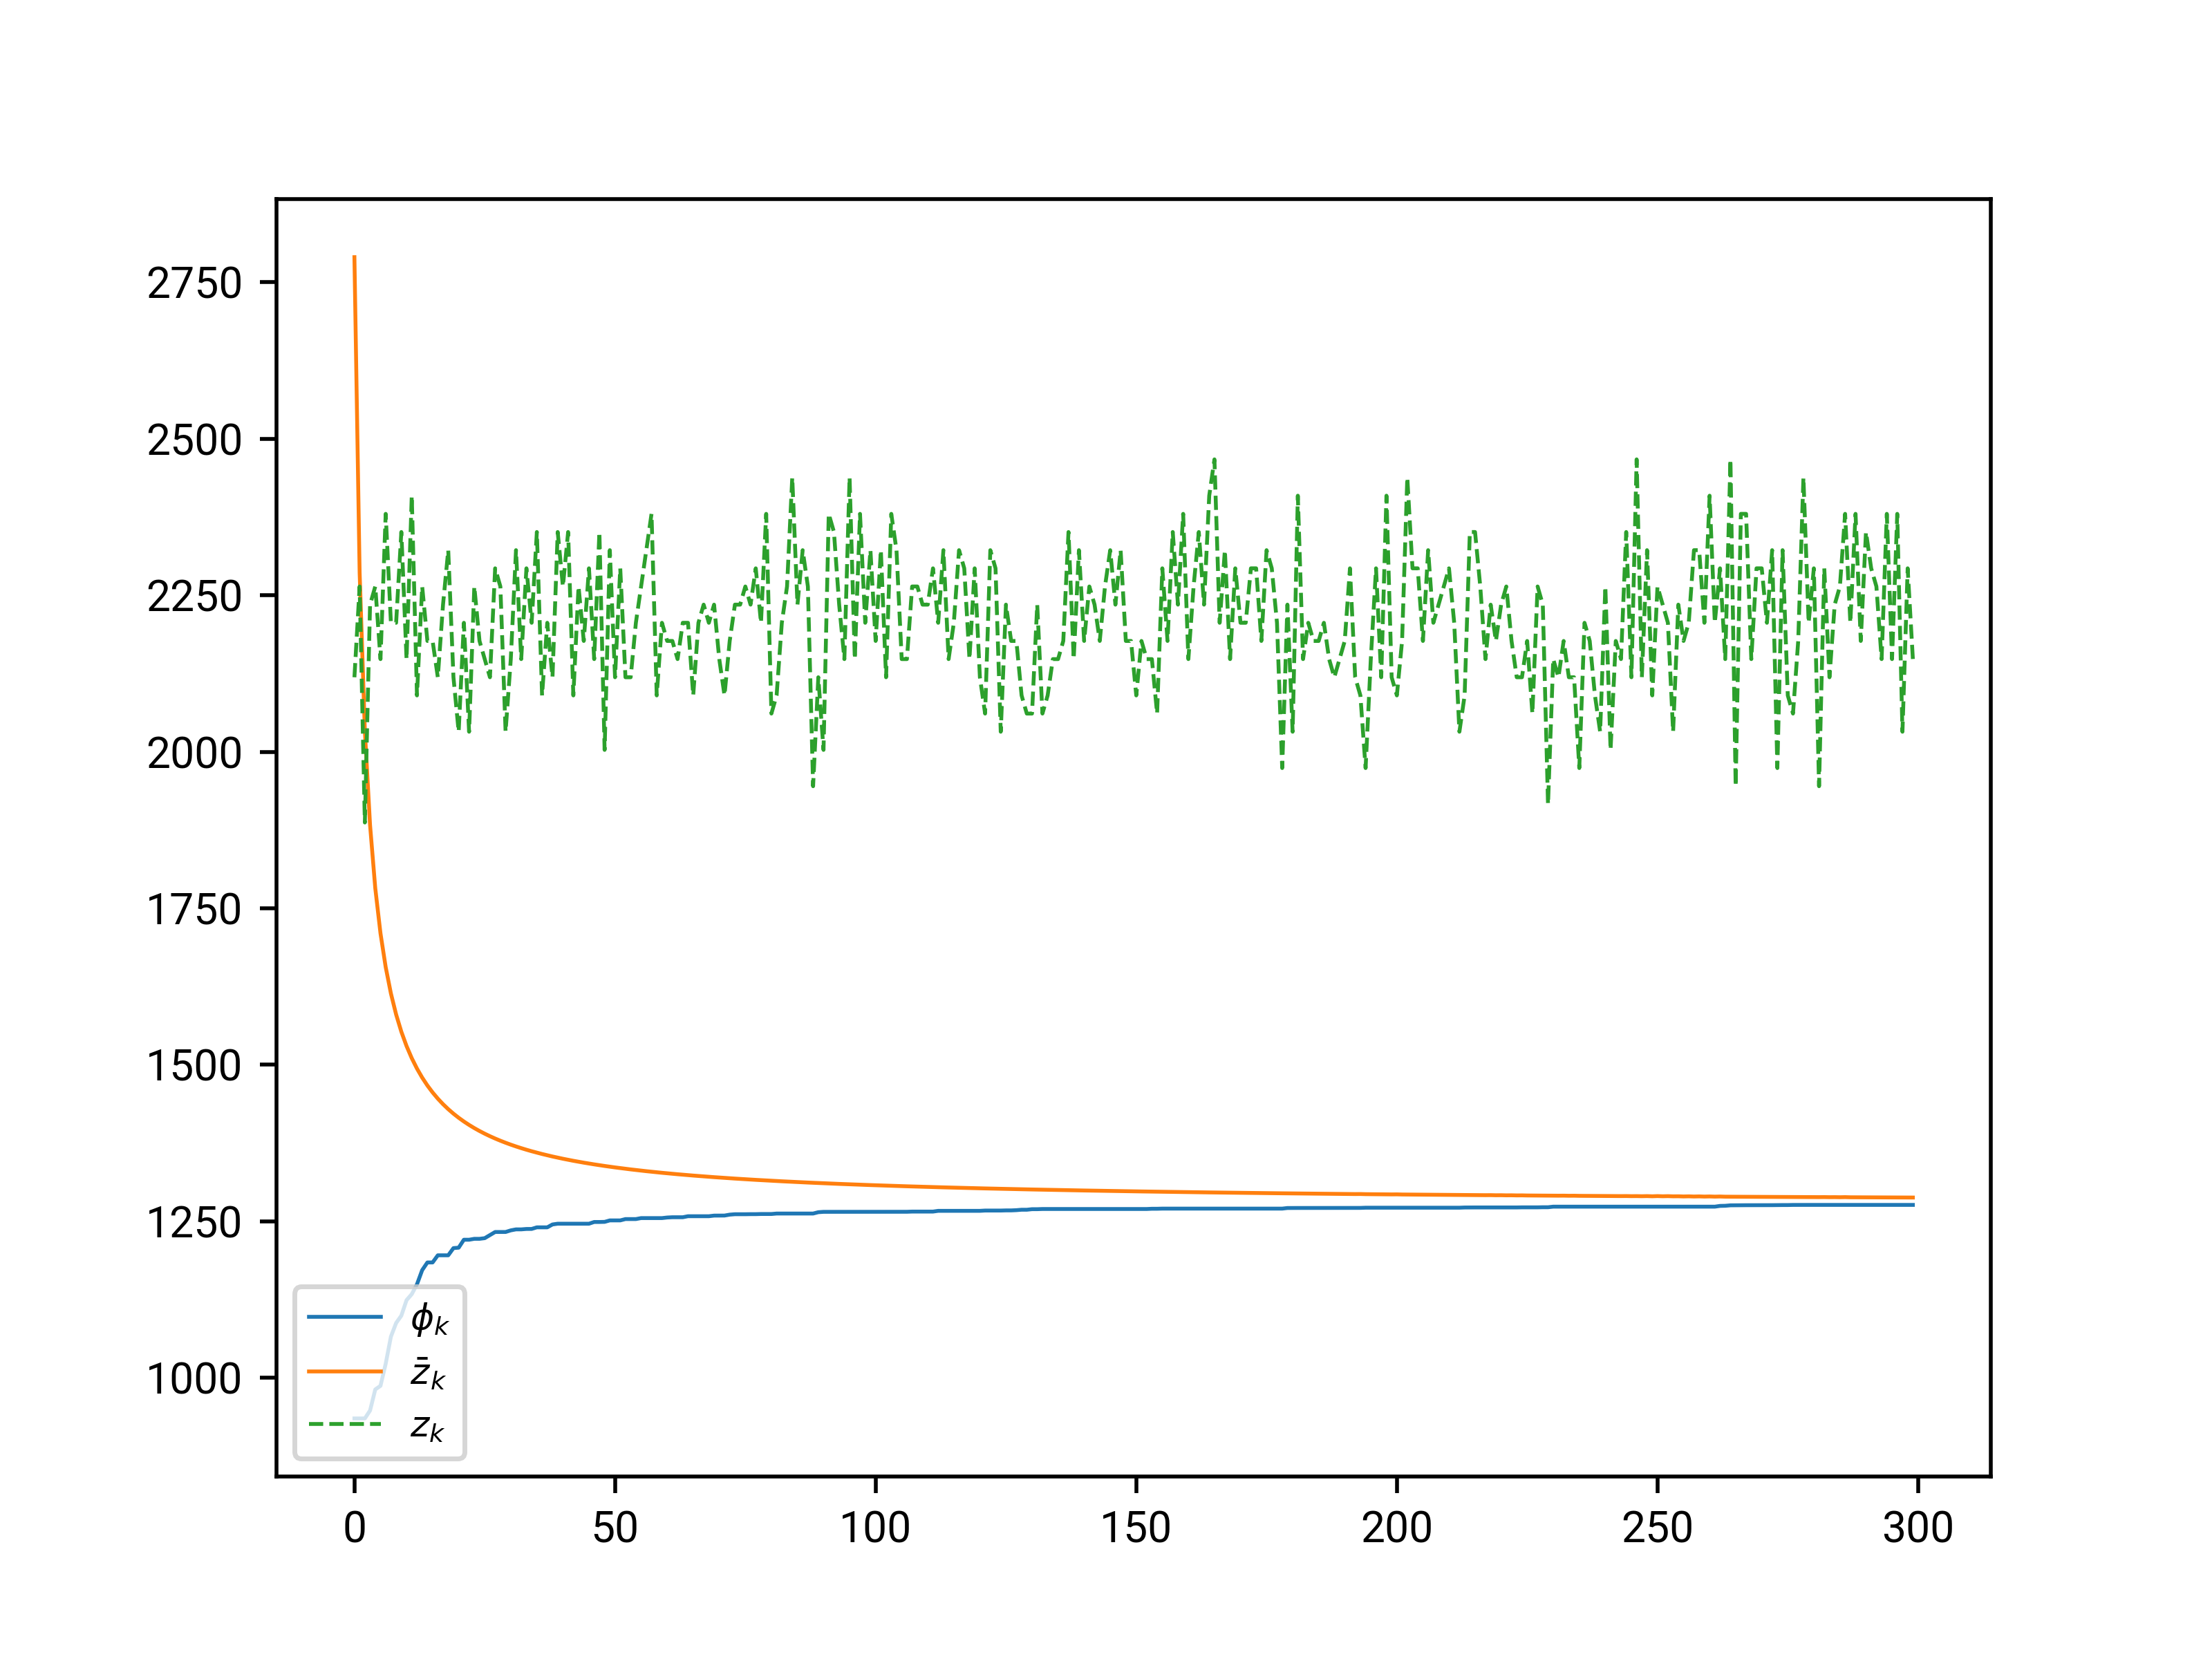
\includegraphics[width=.49\linewidth]{../imgs/conv_0_normal_sg_5_80.png}
  }
  \subfloat[][Convex subgradient method using \(d_k\)]{
    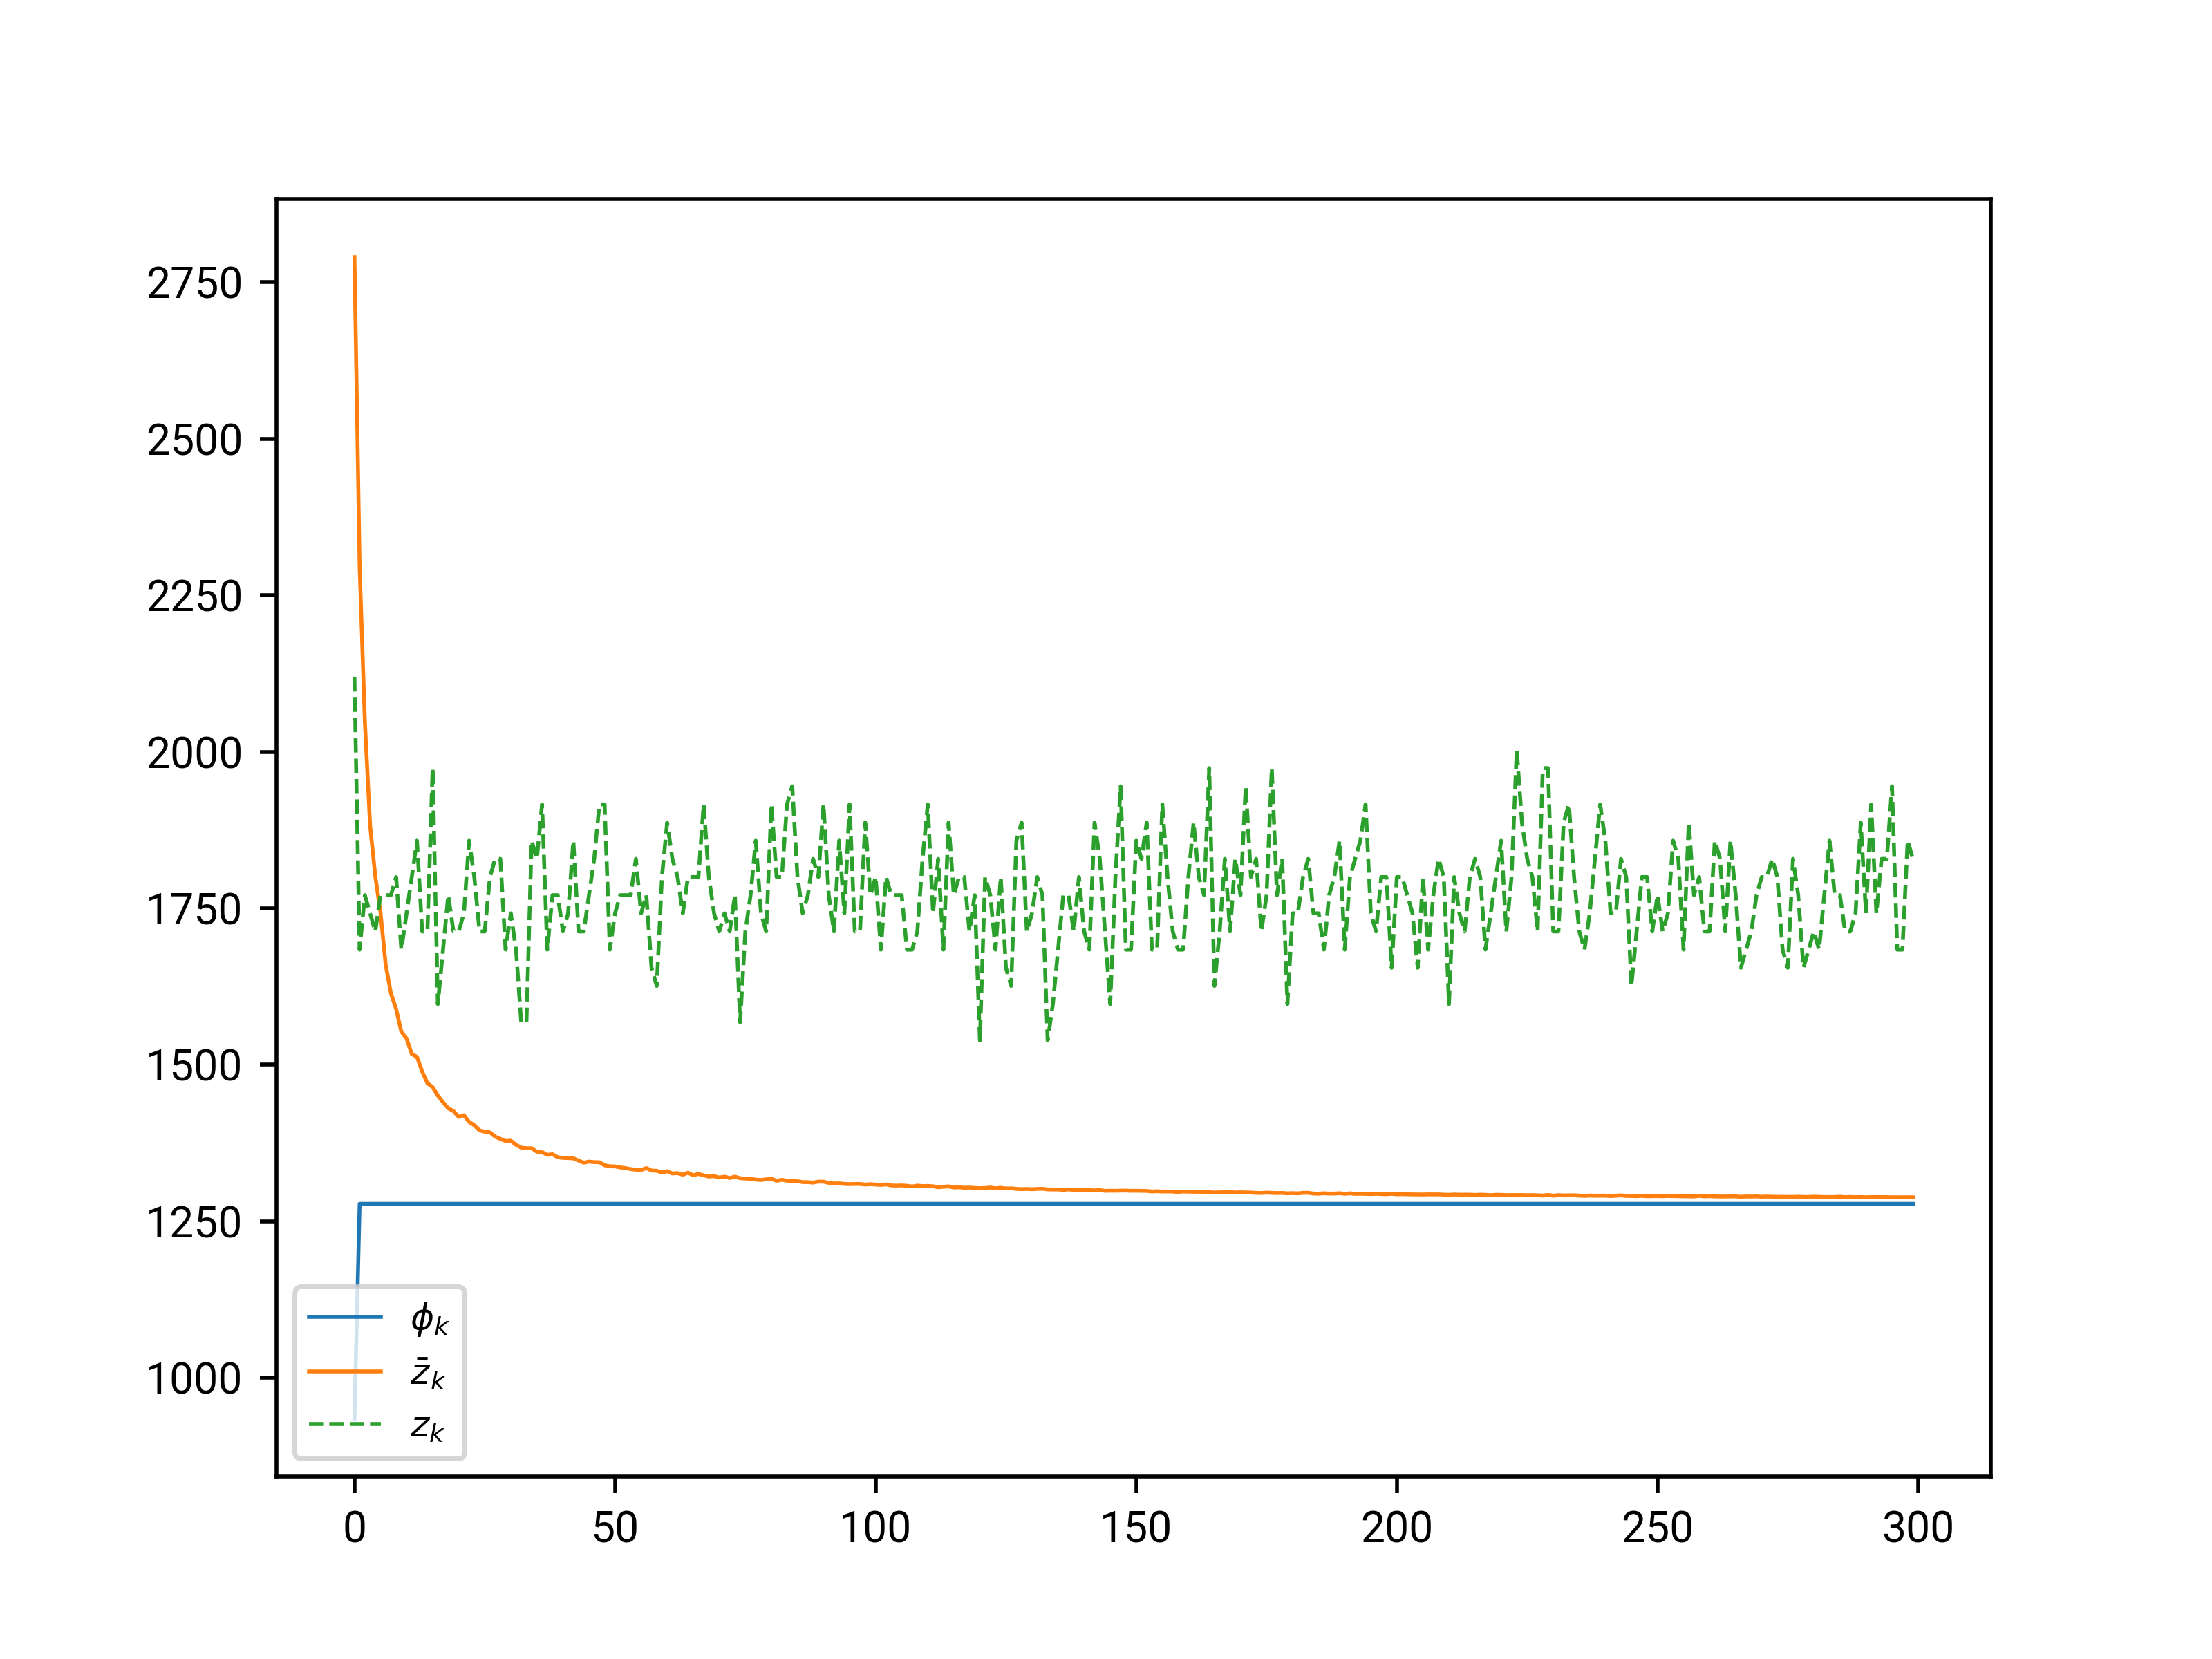
\includegraphics[width=.49\linewidth]{../imgs/conv_0_convex_sg_5_80.png}
  }

  \caption{
    An instance illustrating the convergence of the subgradient methods
    and the recovery algorithm \eqref{eq:recovery}.
    \(\phi_k\) and \(\bar z_k\) are lower bound for the subgradient method
    and averaged primal value from the recovery algorithm, respectively.
    \(z_k\) is the primal value at iteration \(k\) without averaging.
    We find that averaged solution avoids the zig-zag behavior of \(z_k\).
  }

  \label{fig:divergent_volume}
\end{figure}


We summarize all test cases in Table \ref{tab:comp_repair_cases}.


\end{document}